\documentclass[hidelinks,12pt]{article}
\usepackage{graphicx}
\usepackage{layout}
\usepackage{amsmath, amssymb}
\usepackage{hyperref}
\usepackage{float}
\usepackage{fancyhdr}
\usepackage{titlesec}
\usepackage[dvipsnames]{xcolor}
\usepackage{lipsum}
\usepackage{cleveref}
\usepackage[a4paper,left=3cm,right=2cm,top=2.5cm,bottom=2.5cm]{geometry}
\usepackage{overpic}
\usepackage{booktabs}
\usepackage{subcaption}
\usepackage{titlesec}
\usepackage{caption}
\usepackage{lipsum}
\usepackage{enumitem}

\pagestyle{fancy}
\fancyhf{}
% \renewcommand{\headrulewidth}{0pt}
\cfoot{\thepage}

\setlength{\parindent}{0pt}

\graphicspath{ {./figs/} }

\author{M.M. Roshani}

\begin{document}
	\begin{titlepage}
		\begin{center}
			\begin{figure}
				\vspace{-1.0cm}
				\centering
				
\includegraphics[scale=0.35]{SUT_logo}
			\end{figure}
			\mbox{}\\[2.0cm]
			\textsc{\Huge \textbf{Signals and Systems Project}}\\[1.0cm]
			\textsc{\LARGE Phase 2}\\[1.5cm]
			\textsc{\LARGE Instructor: Prof. Hamid Aghajan}\\[1cm]
			\textsc{\LARGE Sharif University of Technology}\\[1.0cm]
			\rule{\linewidth}{0.5mm} \\
			{\large \bf {\fontfamily{cmss}\selectfont Analysis of Phase-Amplitude Coupling during Olfactory Stimulation \\ \medskip as a Biomarker for Alzheimer's Disease in EEG Signals}}\\[0.2cm]
			\rule{\linewidth}{0.5mm} \\
			\vfill
			{\Large M.M. Roshani}
		\end{center}
	\end{titlepage}
	
	\tableofcontents
	\newpage
	
	
	\section{Introduction}
	\subsection{Understanding Modulation and Phase-Amplitude Coupling}
	
	In neuroscience, modulation refers to a statistical relationship describing how the properties of one brain oscillation influence those of another. This can be understood through a simple analogy:
	
	\begin{itemize}
	\item The \textbf{modulating signal} can be imagined as a slow, consistent, repeating rhythm, like a drumbeat. This represents the phase of the slow theta wave (4--8 Hz), which indicates its exact position in its cycle at any given moment.
	
	\item The \textbf{modulated signal} can be thought of as a rapid, flickering light that gets consistently brighter or dimmer. This represents the amplitude of the fast gamma wave (30--50 Hz).
	\end{itemize}
	
	This relationship means the gamma amplitude is dependent on the theta phase. We can confirm modulation when the fast-flickering light consistently gets brighter at a specific point in the slow drumbeat's cycle.
	\bigbreak
	Specifically, this process is known as Phase-Amplitude Coupling (PAC). PAC analyzes how the brightness (amplitude) of the fast gamma wave is directly linked to the rhythm (phase) of the slow theta wave. For instance, the gamma amplitude might always peak when the theta wave is at its trough, corresponding to the $-\pi$ phase on a circular representation.
	
	\subsection{Methods for Measuring PAC}
	
	To measure PAC, we must first filter the raw brain signal to extract the phase of the slow theta wave and the amplitude of the fast gamma wave. Once these are obtained, their relationship can be quantified using two primary methods:
	
	\begin{itemize}
		\item \textbf{Modulation Vector Length (MVL):} This method plots gamma amplitudes as points on a circular compass based on the theta phase. If the gamma amplitude consistently clusters at a particular phase, the resulting average vector will be longer (closer to a value of 1), indicating strong coupling.
		
		\item \textbf{Modulation Index (MI):}  This method divides the theta cycle into sections, or "bins," and measures the total gamma amplitude within each bin. If the gamma amplitude is not tied to the theta phase, the distribution will be flat. A strong relationship, however, will create a clear peak in the distribution, and the MI value quantifies the size of this peak.
	\end{itemize}
	
	\newpage
	
	
	\begin{figure}[h!]
		\centering
		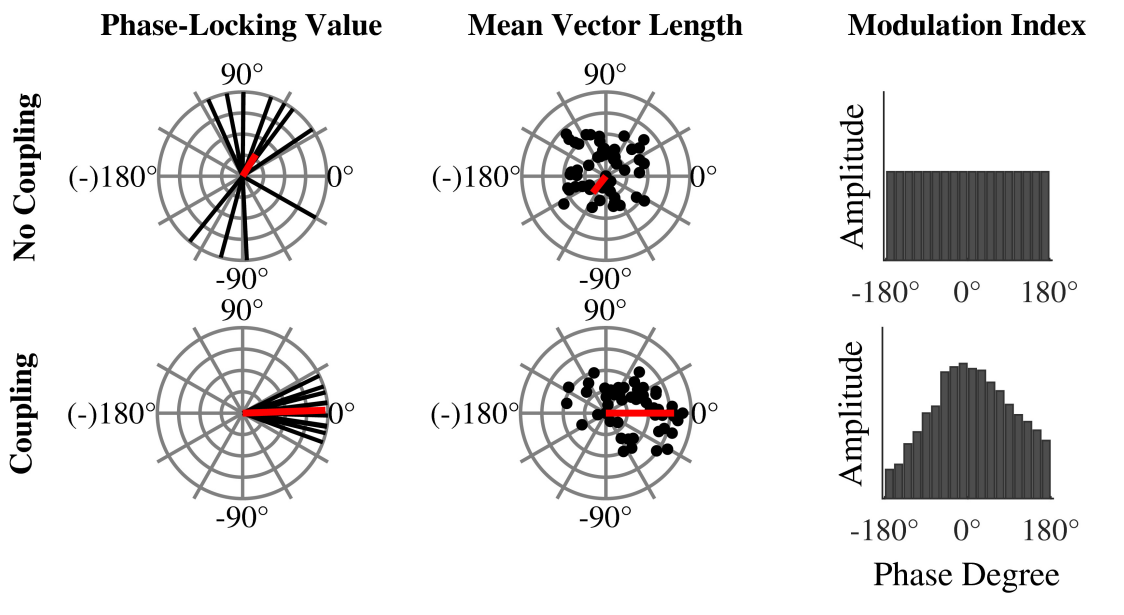
\includegraphics[width=0.7\textwidth]{1}
		\caption[Caption for LOF]{MVL and MI representation\footnotemark}
	\end{figure}
	\footnotetext{From an \href{https://www.frontiersin.org/journals/neuroscience/articles/10.3389/fnins.2019.00573/full}{\textcolor{cyan}{article}} on Frontiers}
	
	
	\subsection{How the Wavelet Transform Helps}
	To measure the amplitude of the gamma wave at a specific phase of the theta wave, we need a tool that can analyze both the time and frequency domains simultaneously. While the Fourier Transform is a useful tool for a frequency-based analysis, it does not provide us with the necessary time-based information. This is due to a fundamental trade-off: to get a precise view of frequency, we must sacrifice the precision of time. The wavelet transform solves this problem by balancing this trade-off. It provides a high time resolution for high frequencies (like the gamma wave), which are often brief, and a high frequency resolution for low frequencies (like the theta wave), which last longer.
	
	\subsubsection*{An Example} Imagine we're analyzing a traffic light. A Fourier Transform would give the exact same result whether the cycle was "red, yellow, green" or "green, yellow, red," because it loses all information about the order of events.
	
	In contrast, a Wavelet Transform can analyze the signal in small windows, allowing us to see not only what frequencies were present but also when they occurred.

	
	\begin{figure}[h!]
		\centering
		\begin{subfigure}[b]{0.48\textwidth}
			\centering
			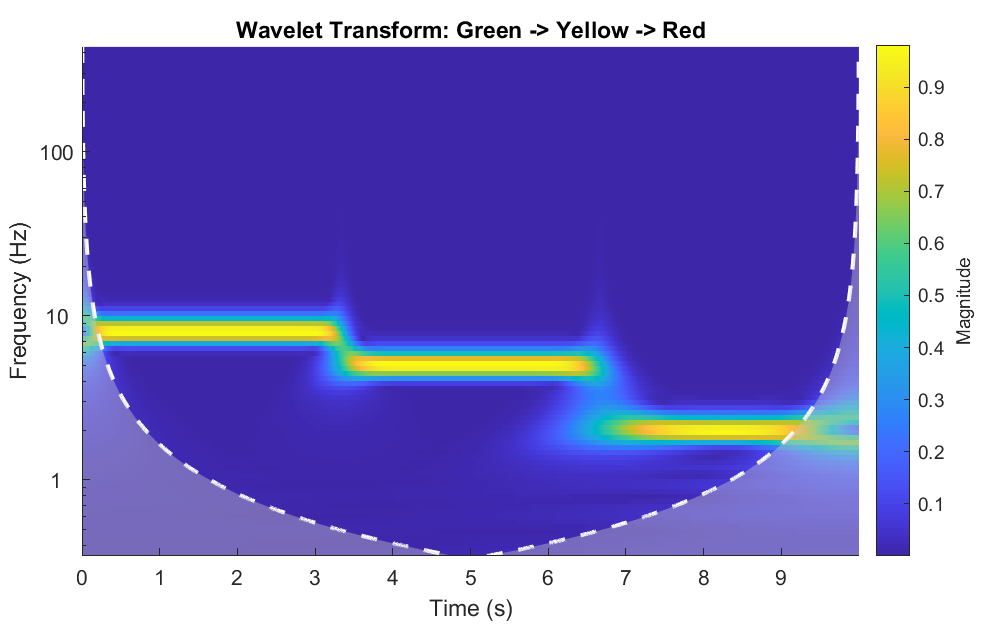
\includegraphics[width=\textwidth]{5}
		\end{subfigure}
		\hfill
		\begin{subfigure}[b]{0.48\textwidth}
			\centering
			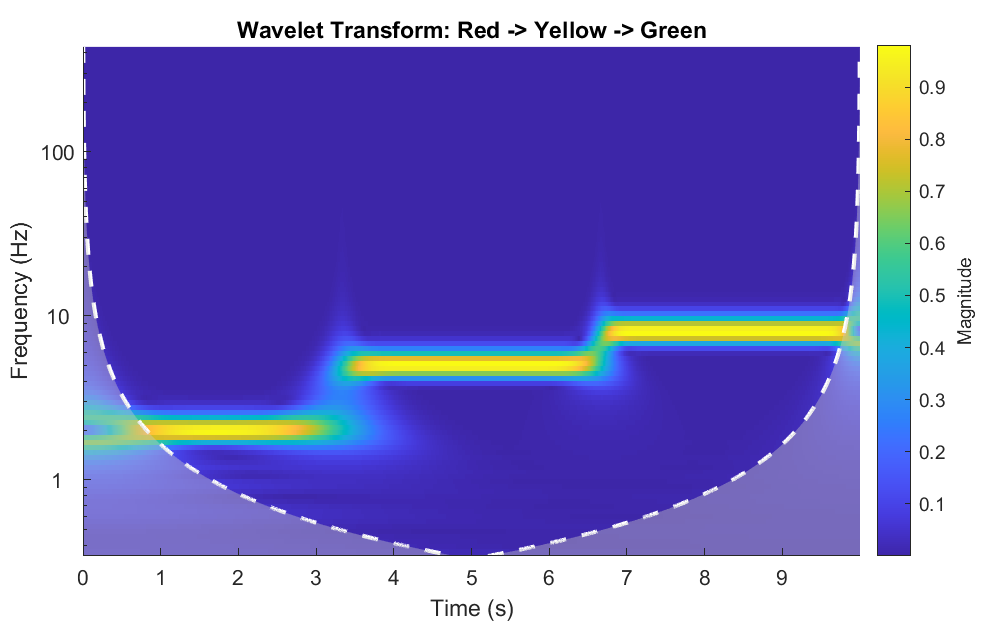
\includegraphics[width=\textwidth]{6}
		\end{subfigure}

	\end{figure}
	
	\newpage
	
	\section{Foundations for PAC Analysis}
	\subsection{Data Preparation and Epoching}
	We began by loading EEG datasets for each condition: Healthy, Mild Cognitive Impairment (MCI), and Alzheimer's Disease (AD). For each group, we identified trials corresponding to specific odors ("Chocolate" and "Rose") using event codes embedded in the data. The continuous data was then segmented into short epochs aligned to the onset of each odor presentation. This process resulted in a separate epoched dataset for each group-odor combination.
	
	\subsection{Time-Frequency Analysis}
	
	To begin the analysis, we applied the continuous wavelet transform to the raw EEG signal for each trial and channel, generating a complete time-frequency decomposition across a wide range of frequencies. From the resulting matrix of wavelet coefficients, we then performed frequency-band selection to isolate the data for the theta wave (4--8 Hz) and the gamma wave (30--50 Hz). Finally, the instantaneous phase of the theta wave was calculated by averaging the wavelet coefficients within its frequency band and taking the angle of the result. Similarly, the instantaneous amplitude of the gamma wave was obtained by averaging the magnitude of the wavelet coefficients within its band.
	
	\subsection{Constructing the Complex Z-Vector}
	
	We then created a time series called the $z$ vector for each trial and channel. This vector is designed to represent two key pieces of information at once: it encodes the gamma amplitude in its magnitude and the theta phase in its angle.
	
	\[
	z(t) = A_\gamma(t) e^{i \phi_\theta(t)}
	\]
	
	Here, $A_\gamma(t)$ is the gamma amplitude at any given moment, and $\phi_\theta(t)$ is the corresponding theta phase. This representation allowed us to capture how the theta phase continuously influences the gamma amplitude, providing a foundation for all our subsequent calculations on PAC.
	
	\begin{figure}[bh!]
		\centering
		
		\begin{subfigure}[b]{0.3\textwidth}
			\centering
			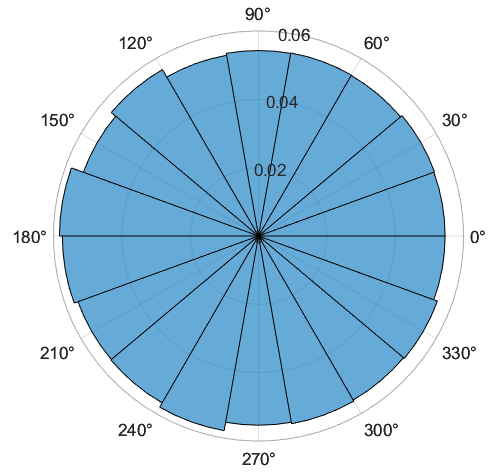
\includegraphics[width=\textwidth]{7}
			\caption{Healthy}
		\end{subfigure}
		\hfill
		\begin{subfigure}[b]{0.3\textwidth}
			\centering
			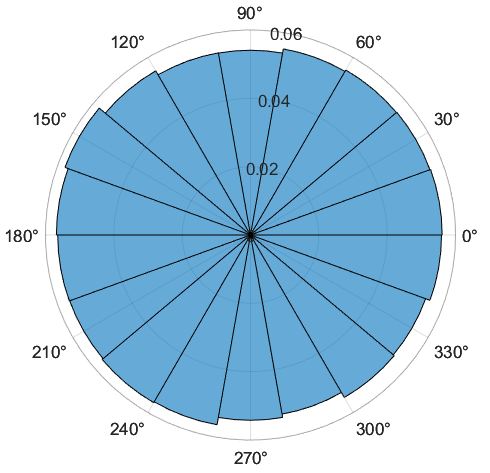
\includegraphics[width=\textwidth]{8}
			\caption{MCI}
		\end{subfigure}
		\hfill
		\begin{subfigure}[b]{0.3\textwidth}
			\centering
			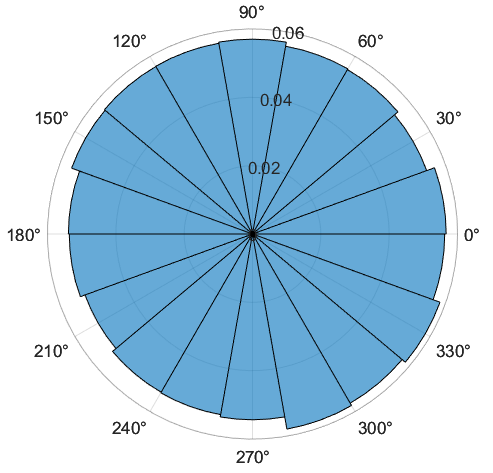
\includegraphics[width=\textwidth]{9}
			\caption{AD}
		\end{subfigure}
		
		\caption{Phase distribution for chocolate odor}
	\end{figure}
	
	
	\newpage
	
	\section{MVL Calculation}
	\subsection{Methodology}
	To quantify the PAC, we first computed the Mean Vector Length (MVL) for each trial and channel from the $z$ vector using the formula
	\[
	MVL = \left| \frac{1}{T} \sum_{t} z(t) \right|,
	\]
	which gives a single value representing the strength of coupling. The calculation was performed in the following steps:
	\begin{enumerate}
		\item Average across channels to obtain one MVL value per trial.
		\item Average across trials to obtain one MVL value per condition (group $\times$ odor).
	\end{enumerate}
	
	In addition to this single-value analysis, we also performed a time-resolved MVL analysis using a sliding window of 1 second with a 95\% overlap. This allowed us to examine how the MVL changed over the course of each trial.
	\bigbreak
	Finally, to understand the variability of our results, we computed the Standard Deviation (SD) of these MVL values across all trials for a given condition. This gave us a single number that quantified how much the MVL varied from one trial to the next.
	
	
	\subsection{Results and Interpretation}
	
	
	\begin{figure}[h!]
		\centering
		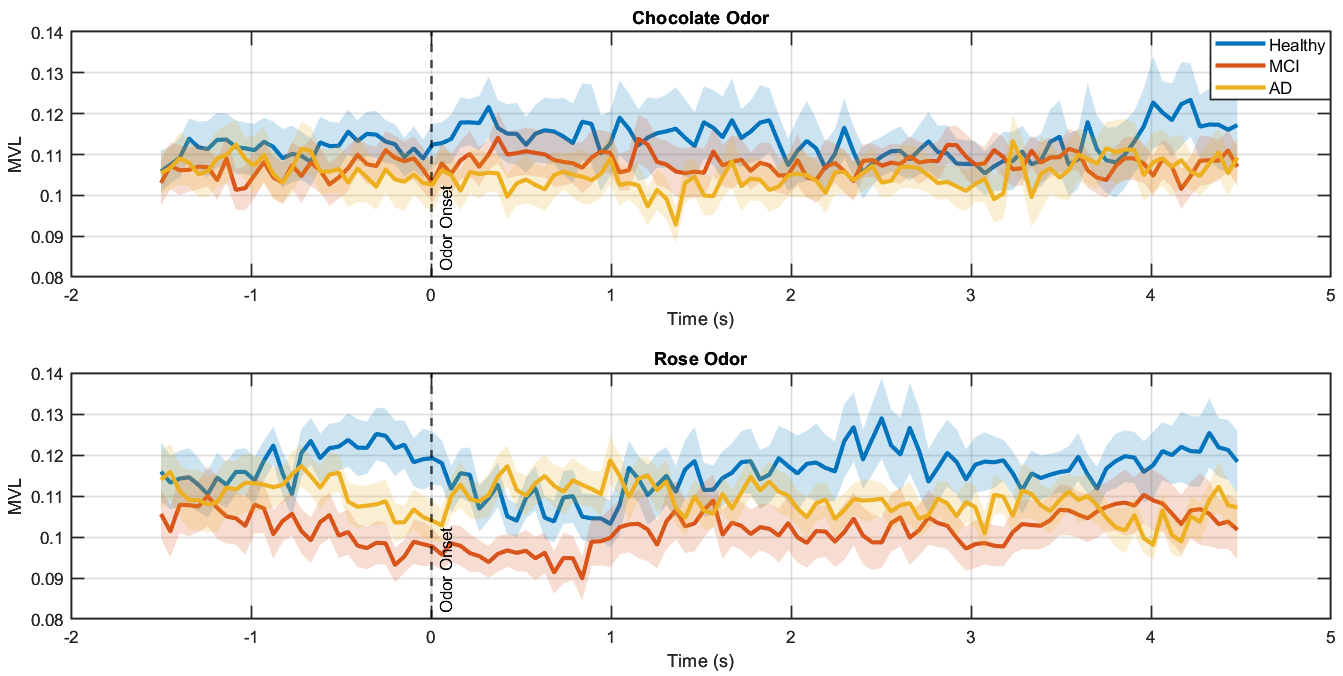
\includegraphics[width=\textwidth]{10}
		\caption{Time-Resolved MVL by group and odor}
	\end{figure}
	
	\newpage
	
	\begin{table}[h!]
		\centering
		\begin{tabular}{lcc}
			\hline
			\textbf{Condition} & \textbf{Chocolate} & \textbf{Rose} \\
			\hline
			Healthy & 0.04026 & 0.04584 \\
			MCI     & 0.03777 & 0.03667 \\
			AD      & 0.03725 & 0.04141 \\
			\hline
		\end{tabular}
		\caption{Overall MVL values}
		\label{table:1}
	\end{table}
	
	\begin{table}[h!]
		\centering
		\begin{tabular}{lcc}
			\hline
			\textbf{Condition} & \textbf{Chocolate} & \textbf{Rose} \\
			\hline
			Healthy & 0.0347 & 0.0462 \\
			MCI     & 0.0236 & 0.0421 \\
			AD      & 0.0319 & 0.0374 \\
			\hline
		\end{tabular}
		\caption{Coefficient of variation (CV) of MVL}
		\tiny{Values represent CV calculated across sliding windows over time.}
		\label{table:2}
	\end{table}
	
	
	\begin{itemize}
		\item[$\blacksquare$] Does PAC increase during stimulus delivery, and does it serve to distinguish between cognitive states?
		
		Our analysis of the olfactory data reveals that PAC-measured brain activity differs between healthy individuals and those with cognitive impairment.
		
		\begin{itemize}
			\item \textbf{Chocolate Odor}: All groups show an increase in PAC following the odor's onset, indicating that the brain is actively responding to the stimulus. The strength of this response, however, progressively diminishes across the groups. This suggests the ability to generate a robust PAC signal in response to a pleasant, non-soothing stimulus appears to be associated with cognitive health.
			
			\item \textbf{Rose Odor}: The response highlights a difference in the pattern of brain activity, which suggests that the pattern of the PAC response is more informative than its magnitude alone. Both the Healthy and MCI groups show a unique response, with an initial drop in PAC at odor onset followed by an increase. In contrast, the AD group does not exhibit this initial drop; their response is a relatively flat line with no significant change in its pattern. This qualitative difference suggests that a specific neural mechanism, potentially related to a soothing response, is present in healthy and MCI brains but appears to be impaired in the AD brain.
		\end{itemize}
		

		
		
		
		\item[$\blacksquare$] Are coupling dynamics consistent across trials and subjects?
		
		To assess the reliability of our MVL findings, we calculated a time-resolved coefficient of variation (CV) for the MVL data. This was done using a 1-second sliding window with a 95\% overlap. We then averaged the CV across time to obtain a single reliability score for each condition. As shown in Table~\ref{table:2}, all CV values were relatively low, remaining below 10\%. While there is no universally established cutoff specific to EEG data, values in this range are generally interpreted as reflecting low variability and good consistency across trials.
		
		
		

		
	\end{itemize}
	
	\newpage
	
	\section{Modulation Index (MI) Analysis}
	
	\subsection{Methodology}
	
	To quantify PAC using the Modulation Index (MI), the theta phase range of $[-\pi, \pi]$ was first divided into $n = 18$ equally spaced bins. For each bin, the mean gamma amplitude was computed over all time points where the theta phase fell into that bin, resulting in a distribution of amplitudes across phase bins.  
	\bigbreak
	The MI was then calculated as the normalized Kullback--Leibler divergence between this observed distribution and a uniform one, as shown in the formula:
	
	
	\[
	MI = \frac{D_{KL}(P(\theta) \parallel U(\theta))}{\log(n)}
	\]
	
	Here, $D_{\mathrm{KL}}$ is a measure of how one probability distribution differs from a uniform distribution $U(\theta)$, and $P(\theta)$ is the distribution of gamma amplitudes across the phase bins. A higher MI value indicates a greater deviation from a uniform distribution, signifying stronger PAC.  
	\bigbreak
	To quantify PAC, we first calculated a single MI value for each trial by averaging the MI values across all channels. These per-trial MI values were then averaged to obtain a single MI value for each group and odor condition. Finally, to analyze the MI dynamics within a trial, a sliding window of 1 second with a 95\% overlap was applied. For each window, the MI was computed per channel and then averaged across channels and trials to obtain a time-resolved MI estimate. The standard error of the mean (SEM) across trials was also calculated for each window.
	
	
	\subsection{Results and Interpretation}
	
	\begin{figure}[h!]
		\centering
		\begin{subfigure}[b]{0.85\textwidth}
			\centering
			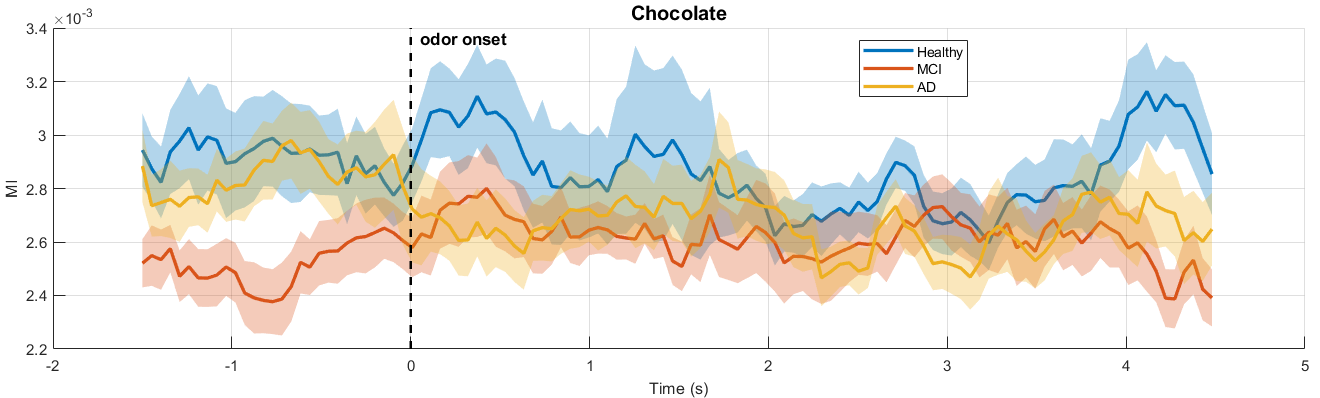
\includegraphics[width=\textwidth]{19}
		\end{subfigure}
		\vfill
		\begin{subfigure}[b]{0.85\textwidth}
			\centering
			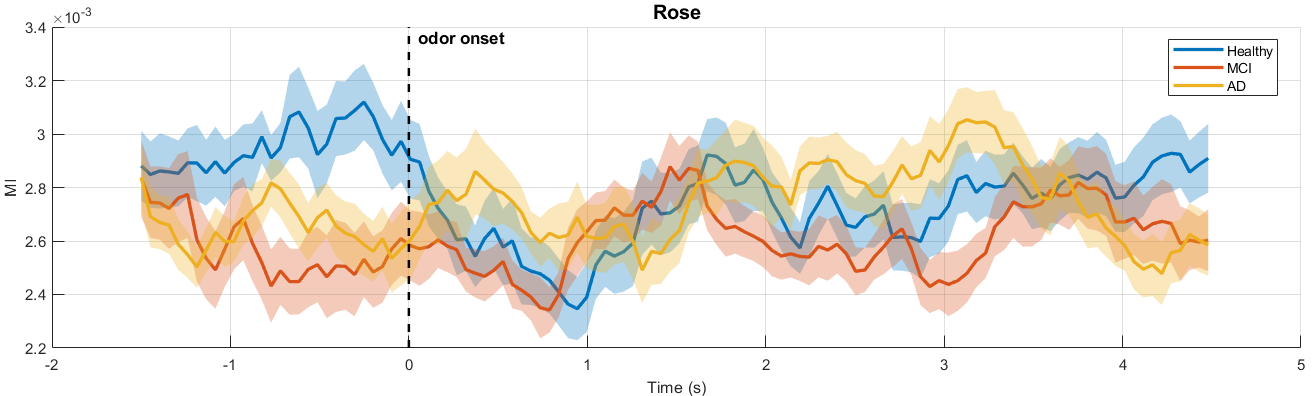
\includegraphics[width=\textwidth]{20}
		\end{subfigure}
		\caption{Time-Resolved MI by group and odor}
	\end{figure}
	\newpage
	\begin{table}[h!]
		\centering
		\begin{tabular}{lcc}
			\hline
			\textbf{Group} & \textbf{Chocolate} & \textbf{Rose} \\
			\hline
			Healthy & 439.27 & 451.04 \\
			MCI     & 380.19 & 382.10 \\
			AD      & 432.52 & 452.27 \\
			\hline
		\end{tabular}
		\caption{MI values ($\times 10^{-6}$) for different groups and stimuli.}
		\label{table:3}
	\end{table}
	
	\begin{itemize}
		\item \textbf{Chocolate Odor}: Following the odor's onset, the Healthy group shows a sustained increase in PAC, suggesting a strong neural response to the stimulus. The MCI group exhibits a similar increase in PAC, but its magnitude is significantly reduced, indicating a diminished capacity for this type of neural processing. In contrast, the AD group displays a fundamentally different response pattern; their MI values remain relatively stable or even show a slight decrease instead of an increase. This provides evidence of a progressive decline in the neural mechanisms for olfactory processing that appears to be correlated with the severity of cognitive impairment.
		
		\item \textbf{Rose Odor}: Following the odor's onset, the Healthy group exhibits a unique response pattern, showing an immediate decrease in MI values followed by a subsequent increase. The MCI group displays a similar response pattern, though it appears to be slightly delayed and less pronounced. The AD group also shows a delayed response, but without the initial decrease. This indicates that while all groups show some form of response to the rose odor, the timing and pattern of this response vary significantly. These qualitative differences offer another potential neural marker for cognitive impairment.
	\end{itemize}

	
	\section{MI vs. MVL}
	While the Modulation Index (MI) and Mean Vector Length (MVL) use different methods to quantify PAC, their time-resolved analyses revealed highly convergent trends.
	\begin{itemize}
		\item \textbf{Chocolate Odor}: For the chocolate odor, both metrics demonstrated consistent patterns. A clear increase in PAC was observed at odor onset across all groups, with the magnitude of this increase being progressively attenuated across the Healthy, MCI, and AD groups. This trend suggests that the magnitude of the PAC response is a potential marker for the severity of cognitive decline.
		
		\item \textbf{Rose Odor}: In the rose odor condition, both MVL and MI analyses revealed a similar pattern of an initial drop in PAC at odor onset for the Healthy and MCI groups. However, the results for the AD group were notably different between the two metrics, indicating that the choice of metric can influence the findings for certain conditions.
		
	\end{itemize}
	In conclusion, the time-resolved analyses of both MVL and MI showed a strong overall alignment in their findings. However, as evidenced by a comparison of Table~\ref{table:1} (MVL) and Table~\ref{table:3} (MI), our analysis suggests that for a single-valued representation of PAC, the MVL method was more effective for distinguishing between cognitive states.
	
	\newpage
	
	\section{PAC analysis with anatomical considerations}
	To examine the consistency of PAC across different brain regions, we conducted a separate analysis on two individual channels: Fp1 and Fp2. These channels, which record data from the orbitofrontal cortex, were selected because this brain region is known to be involved in olfactory processing. Our analysis revealed that the PAC values recorded from these two channels were closely correlated, indicating a high degree of consistency in the neural response to the olfactory stimuli within this specific cortical area.
	
	\begin{figure}[h!]
		\centering
		\begin{subfigure}[b]{0.48\textwidth}
			\centering
			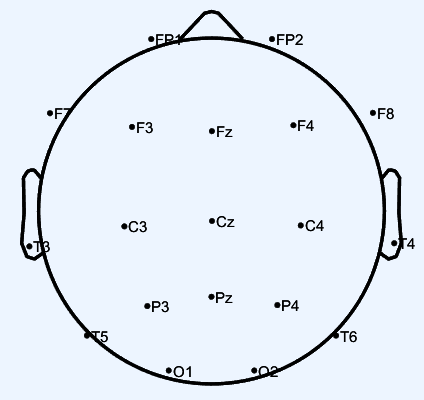
\includegraphics[width=0.6\textwidth]{14}
			\caption*{EEG channel placement on the scalp}
		\end{subfigure}
		\hfill
		\begin{subfigure}[b]{0.48\textwidth}
			\centering
			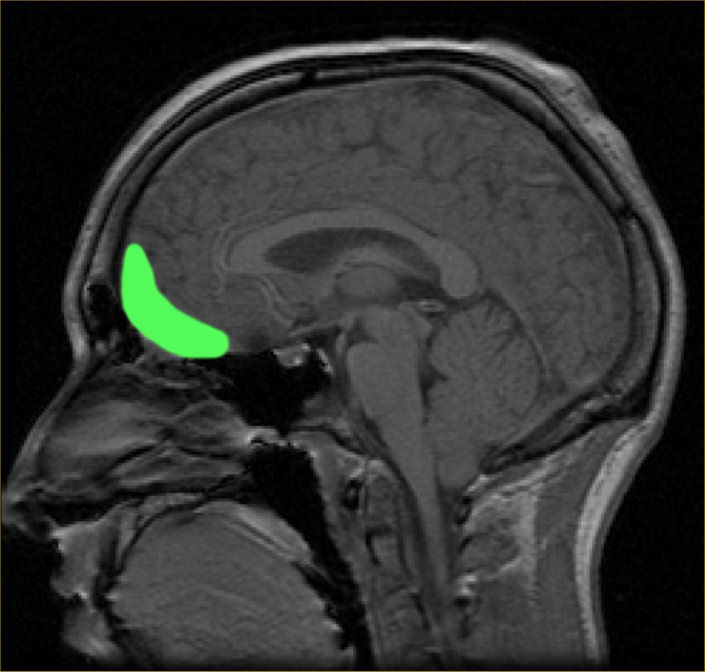
\includegraphics[width=0.6\textwidth]{15}
			\caption*{Orbitofrontal cortex}
		\end{subfigure}
		
	\end{figure}
	

	\begin{figure}[h!]
		\centering
		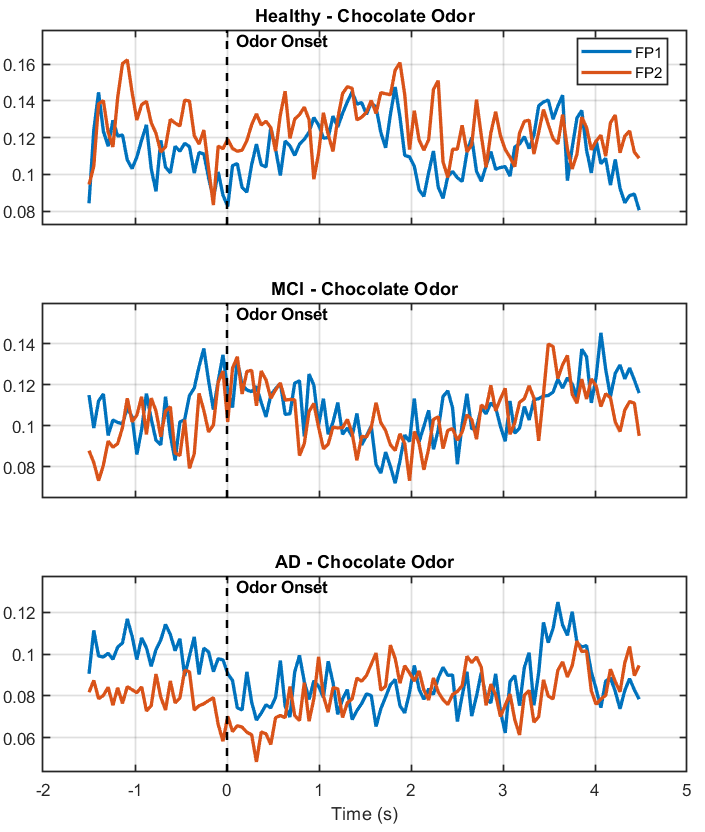
\includegraphics[width=0.65\textwidth]{21}
		\caption{Time-Resolved MVL for Fp1 and Fp2 channels}
	\end{figure}
	
	\newpage
	
	
	Our analysis reveals that in the Healthy and MCI groups, PAC is spatially organized, with recordings from the two channels showing a high degree of alignment. This suggests a consistent neural response within the orbitofrontal cortex in these individuals.
	\bigbreak
	In contrast, this spatial consistency is not observed in the AD group, where there is a noticeable divergence between the recordings from the two channels. This finding suggests that the spatial organization of PAC deteriorates with the progression of cognitive impairment, offering another potential neural marker for the disease.
	
	\section{Additional Visuals}
	The polar histograms of the complex $Z$-vector, $z(t)$, reveal distinct phase-amplitude coupling (PAC) patterns across the groups.  
	\begin{itemize}
		\item The Healthy group exhibits strong coupling, with the gamma amplitude consistently peaking around $230^{\circ}$.  
		
		\item The MCI group shows similar coupling strength, but the peak gamma amplitude is shifted to approximately $180^{\circ}$.  
		
		\item In contrast, the AD group displays a peak PAC at a markedly different phase, around $15^{\circ}$.  
	\end{itemize}
	While the Healthy and MCI groups show a difference in the specific phase where coupling is strongest, the overall timing within the theta cycle remains relatively consistent. The significant shift observed in the AD group suggests a fundamental alteration in the neural timing and coordination between the theta and gamma oscillations.
	
	
	
	\begin{figure}[bh!]
		\centering
		
		\begin{subfigure}[b]{0.3\textwidth}
			\centering
			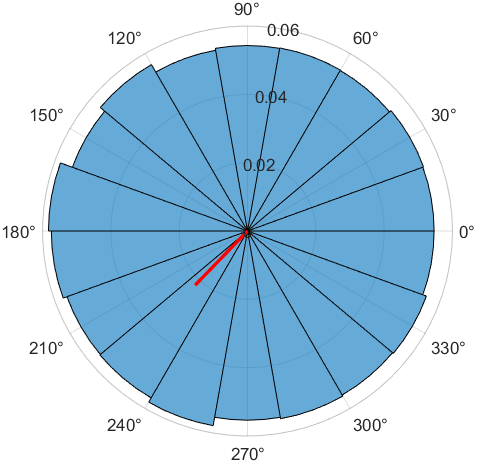
\includegraphics[width=\textwidth]{16}
			\caption{Healthy}
		\end{subfigure}
		\hfill
		\begin{subfigure}[b]{0.3\textwidth}
			\centering
			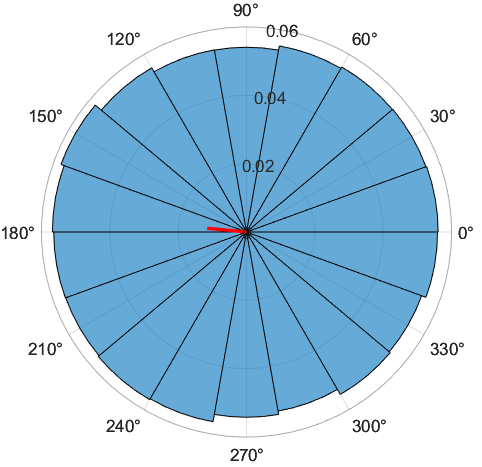
\includegraphics[width=\textwidth]{17}
			\caption{MCI}
		\end{subfigure}
		\hfill
		\begin{subfigure}[b]{0.3\textwidth}
			\centering
			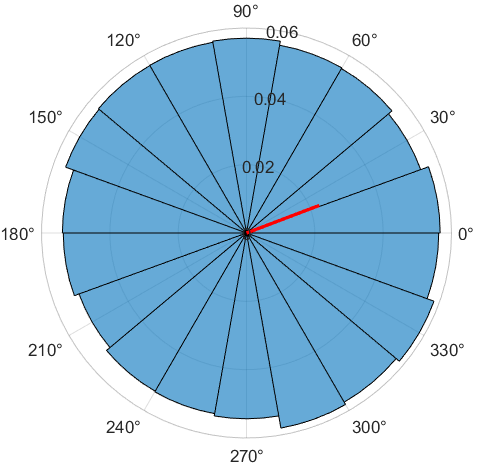
\includegraphics[width=\textwidth]{18}
			\caption{AD}
		\end{subfigure}
		
		\caption{}
	\end{figure}
	
	\newpage

	\section{Conclusion}
	In this phase of the project, our analysis demonstrated that phase-amplitude coupling generally decreases with the progression of cognitive impairment. We observed that the spatial coordination of PAC is also disrupted in the Alzheimer's Disease (AD) group, indicating a breakdown in the neural organization of brain oscillations. Furthermore, the healthier groups exhibited a more timely response to olfactory stimuli compared to the cognitively impaired groups. These findings suggest that PAC metrics, including its magnitude, spatial organization, and temporal dynamics, can serve as potential biomarkers for the severity of cognitive decline.
	
\end{document}
